\documentclass[hidelinks]{article}
\usepackage{tikz}
\usepackage[a4paper,margin=1in]{geometry}
\usepackage{fix-cm}
\usepackage{wrapfig}
\usepackage{float} 
\usepackage{hyperref}
\usepackage{ulem}
\usepackage[document]{ragged2e}
\renewcommand*\familydefault{\sfdefault} 
\pagestyle{plain}

\begin{document}
\vspace*{-5em}
\begin{center}
    \begin{huge}
        Manual of Cyber-physical Systems Lab at Uppsala University\\
    \end{huge}
    \vspace{15pt}
    \begin{large}
        by NIU Xuezhi $<$\href{mailto:xuezhi.niu@it.uu.se}{xuezhi.niu at it.uu.se}$>$
    \end{large}
\end{center}
\vspace*{-1em}

\setlength{\parskip}{13pt plus2pt}
\section*{Overview and available equipments}

\begin{wrapfigure}{r}{0.35\textwidth}
    \begin{center}
        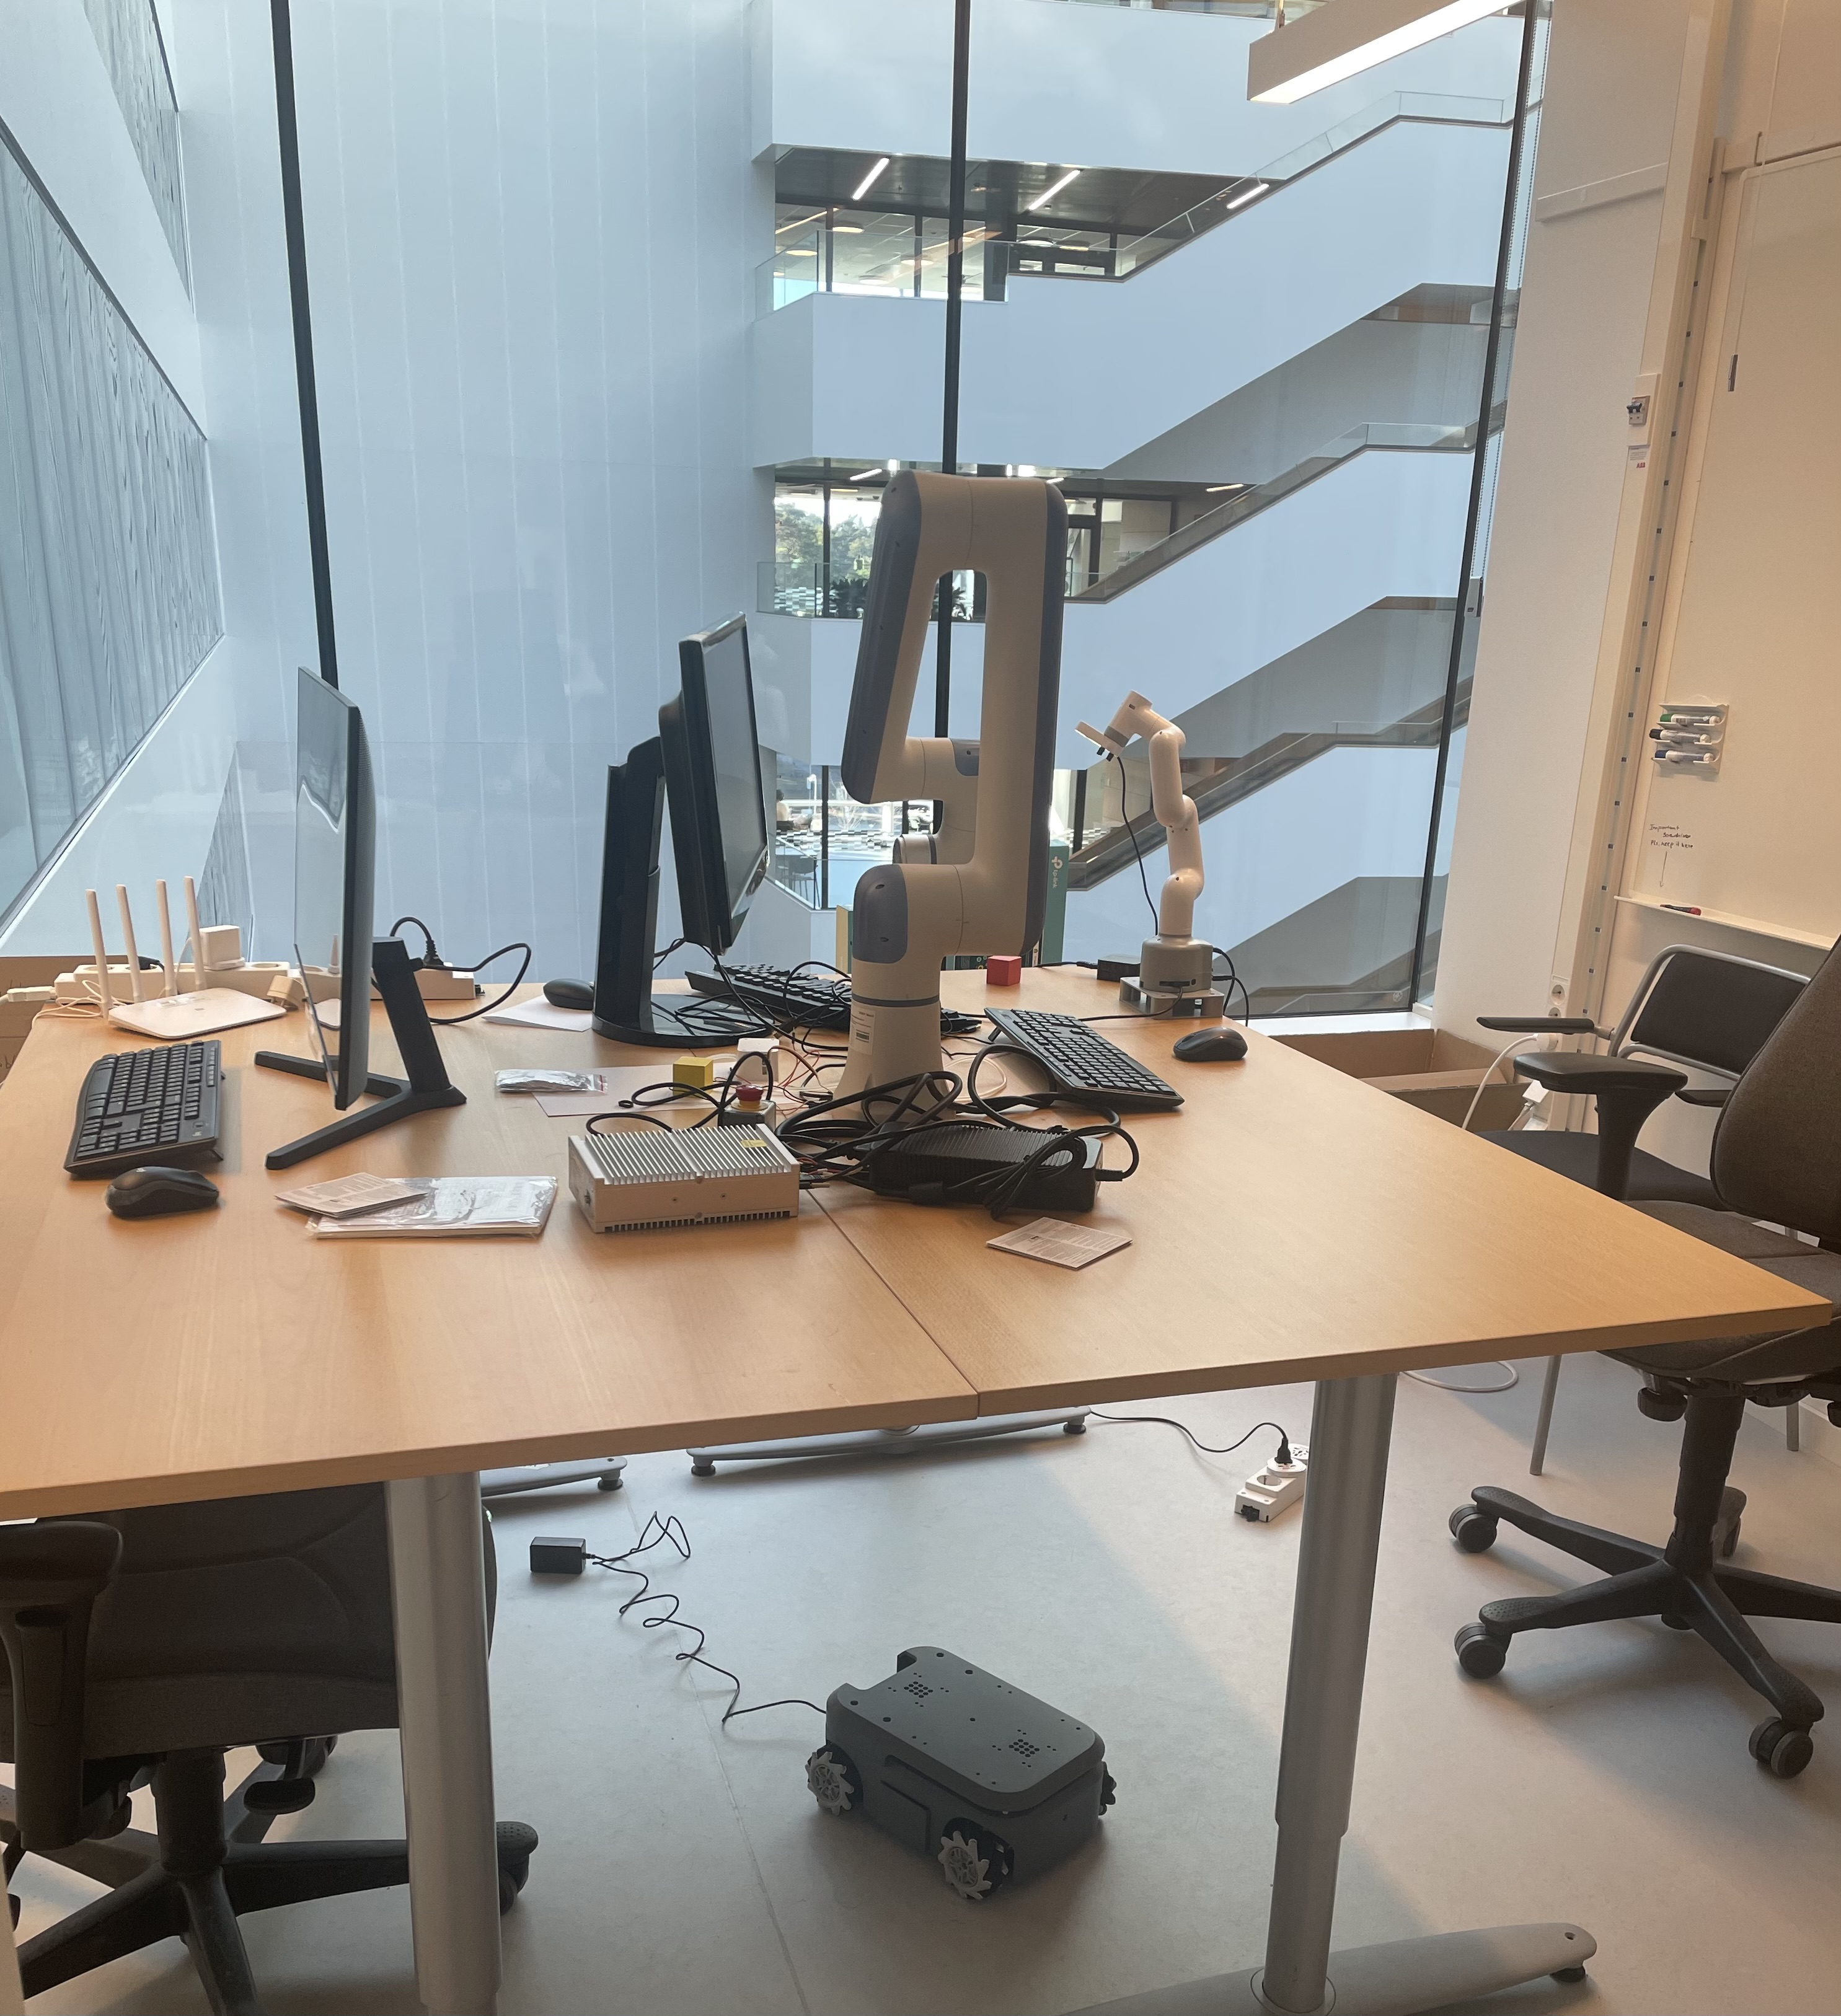
\includegraphics[width=\linewidth]{Figures/MainPhoto.jpeg}
    \end{center}
\end{wrapfigure}

% 
Welcome to the Cyber-Physical Systems Lab at Uppsala University. This manual serves as a guide to understanding the operations, equipment, and protocols within the lab. The Cyber-Physical Lab is dedicated to the exploration, development, and experimentation of systems that integrate computational and physical elements. Our mission is to provide students and researchers with a conducive environment to explore the interdisciplinary field of cyber-physical systems.

Equipment except robots in this lab (up to \today):
\begin{itemize}
    \item Workstation (HP Z2G9 I7-13900K + A4000 \sout{wireless adapter})
    \item TP-Link AX73 Router (Official manual \underline{\href{https://www.tp-link.com/se/support/download/archer-ax73/v2/}{here}})
    \item TP-Link TL-WR841N (Official manual \underline{\href{https://www.tp-link.com/us/user-guides/tl-wr841n_v14/\#ug-sub-title-1}{here}})
    \item Samsung S34C50 Monitor
    \item Kinnarps 6000 Chairs $\times 2$ (Manual \underline{\href{https://www.kinnarps.com/products/seating/task-chairs/60008000/}{here}})
    \item Several Mice and Keyboard from different brands (Wired $\times 2$ + Wireless $\times 2$)
\end{itemize}

As a cyber-physical systems lab, we should have some robots to play with, and implement your genius ideas. However, the foundation of any successful experimentation, especially in a space as interactive and potentially hazardous as ours, is safety. It is crucial to prioritize safety above all.

\subsection*{Lab Safety}
Before we dive into the exciting world of robotics and cyber-physical systems, we must ensure that every lab member is equipped with the knowledge and respect for safety protocols that govern our operations. This commitment to maintaining a secure environment is not just about adhering to rules but about fostering a culture of mindfulness and responsibility towards oneself and others in the lab. 

\textbf{Under no circumstances should any robotic operation be manually interrupted by hand}. Direct physical interaction with moving parts or operational machinery presents a significant risk of injury and can damage the equipment. If there is a need to halt a robot's operation, the first course of action should always be an attempt to interrupt the process via command through the controlling software. If the software fails to respond or an immediate stop is necessary, the next step is to safely power off the equipment. Only after these measures are taken should new operations be initiated.

\textbf{No unattended robotic operations}. It is imperative that robotic operations are not left unattended. When actuating ideas on the robots, your presence is required at all times. This rule ensures that any unexpected issues can be addressed promptly and reduces the risk of accidents or damage to the lab equipment. Unattended operations increase the likelihood of unforeseen incidents, which can lead to potential harm to both the individual and the workspace.

\textbf{Pre-Operation Inspection}. Before initiating any experiment or operation with robotic systems, perform a thorough pre-operation inspection. This includes checking for any signs of wear and tear, ensuring all parts are secured and in their correct positions, and verifying that the software and hardware communication is functioning correctly. Regular inspections help prevent accidents caused by equipment malfunction or failure.

\textbf{Shutdown Before Leaving}. All robotic systems must be properly shut down before leaving the lab. This rule is crucial to prevent any accidental activation or continuation of operations that could occur in the absence of supervision. A powered-down state ensures that the equipment remains safe and secure until it is next used under direct supervision.

\textbf{Also take care of robots}. When working with robots, consider not only your safety but also the well-being of the robots. Abrupt shutdowns or erratic operational commands can lead to wear and tear or even permanent damage to sensitive components. Always shut down the robots gently and as per the recommended procedures when you are done or if you are leaving the lab, even for a short period. This practice extends the lifespan of the robots and maintains their readiness for future experiments.

\subsection*{Robots}
Available Robots in the lab (up to \today):
\begin{itemize}
    \item myCobot 280 Pi $\times 2$ from Elephant Robotics (Official manual \underline{\href{https://docs.elephantrobotics.com/docs/gitbook-en/2-serialproduct/2.1-280/2.1.2-PI.html}{here}})
    \item myAVG $\times 2$ from Elephant Robotics (Official manual \underline{\href{https://docs.elephantrobotics.com/docs/gitbook-en/2-serialproduct/2.5-myAGV.html}{here}})
    \item Nova 5 from Dobot (Official manual \underline{\href{https://www.dobot-robots.com/products/nova-series/nova5.html}{here}})
    \item AI kit 2023 of myCobot from Elephant Robotics (Official manual \underline{\href{https://docs.elephantrobotics.com/docs/gitbook-en/2-serialproduct/2.9-AIkit2023en/introduce.html}{here}})
    \item Gripper RobotiQ 2F85 from Dobot (Official manual \underline{\href{https://robotiq.com/products/2f85-140-adaptive-robot-gripper?ref=nav_product_new_button}{here}})
\end{itemize}

If you want to connect to the robot (except Nova 5), you could try VNC by typing the IP address assigned by the router to have graphical interaction to the ubuntu installed on the robot. There are two ways to get the assigned IP address. This is what you can achieve, as shown in the figure below.

\begin{figure}[H]
    \centering
    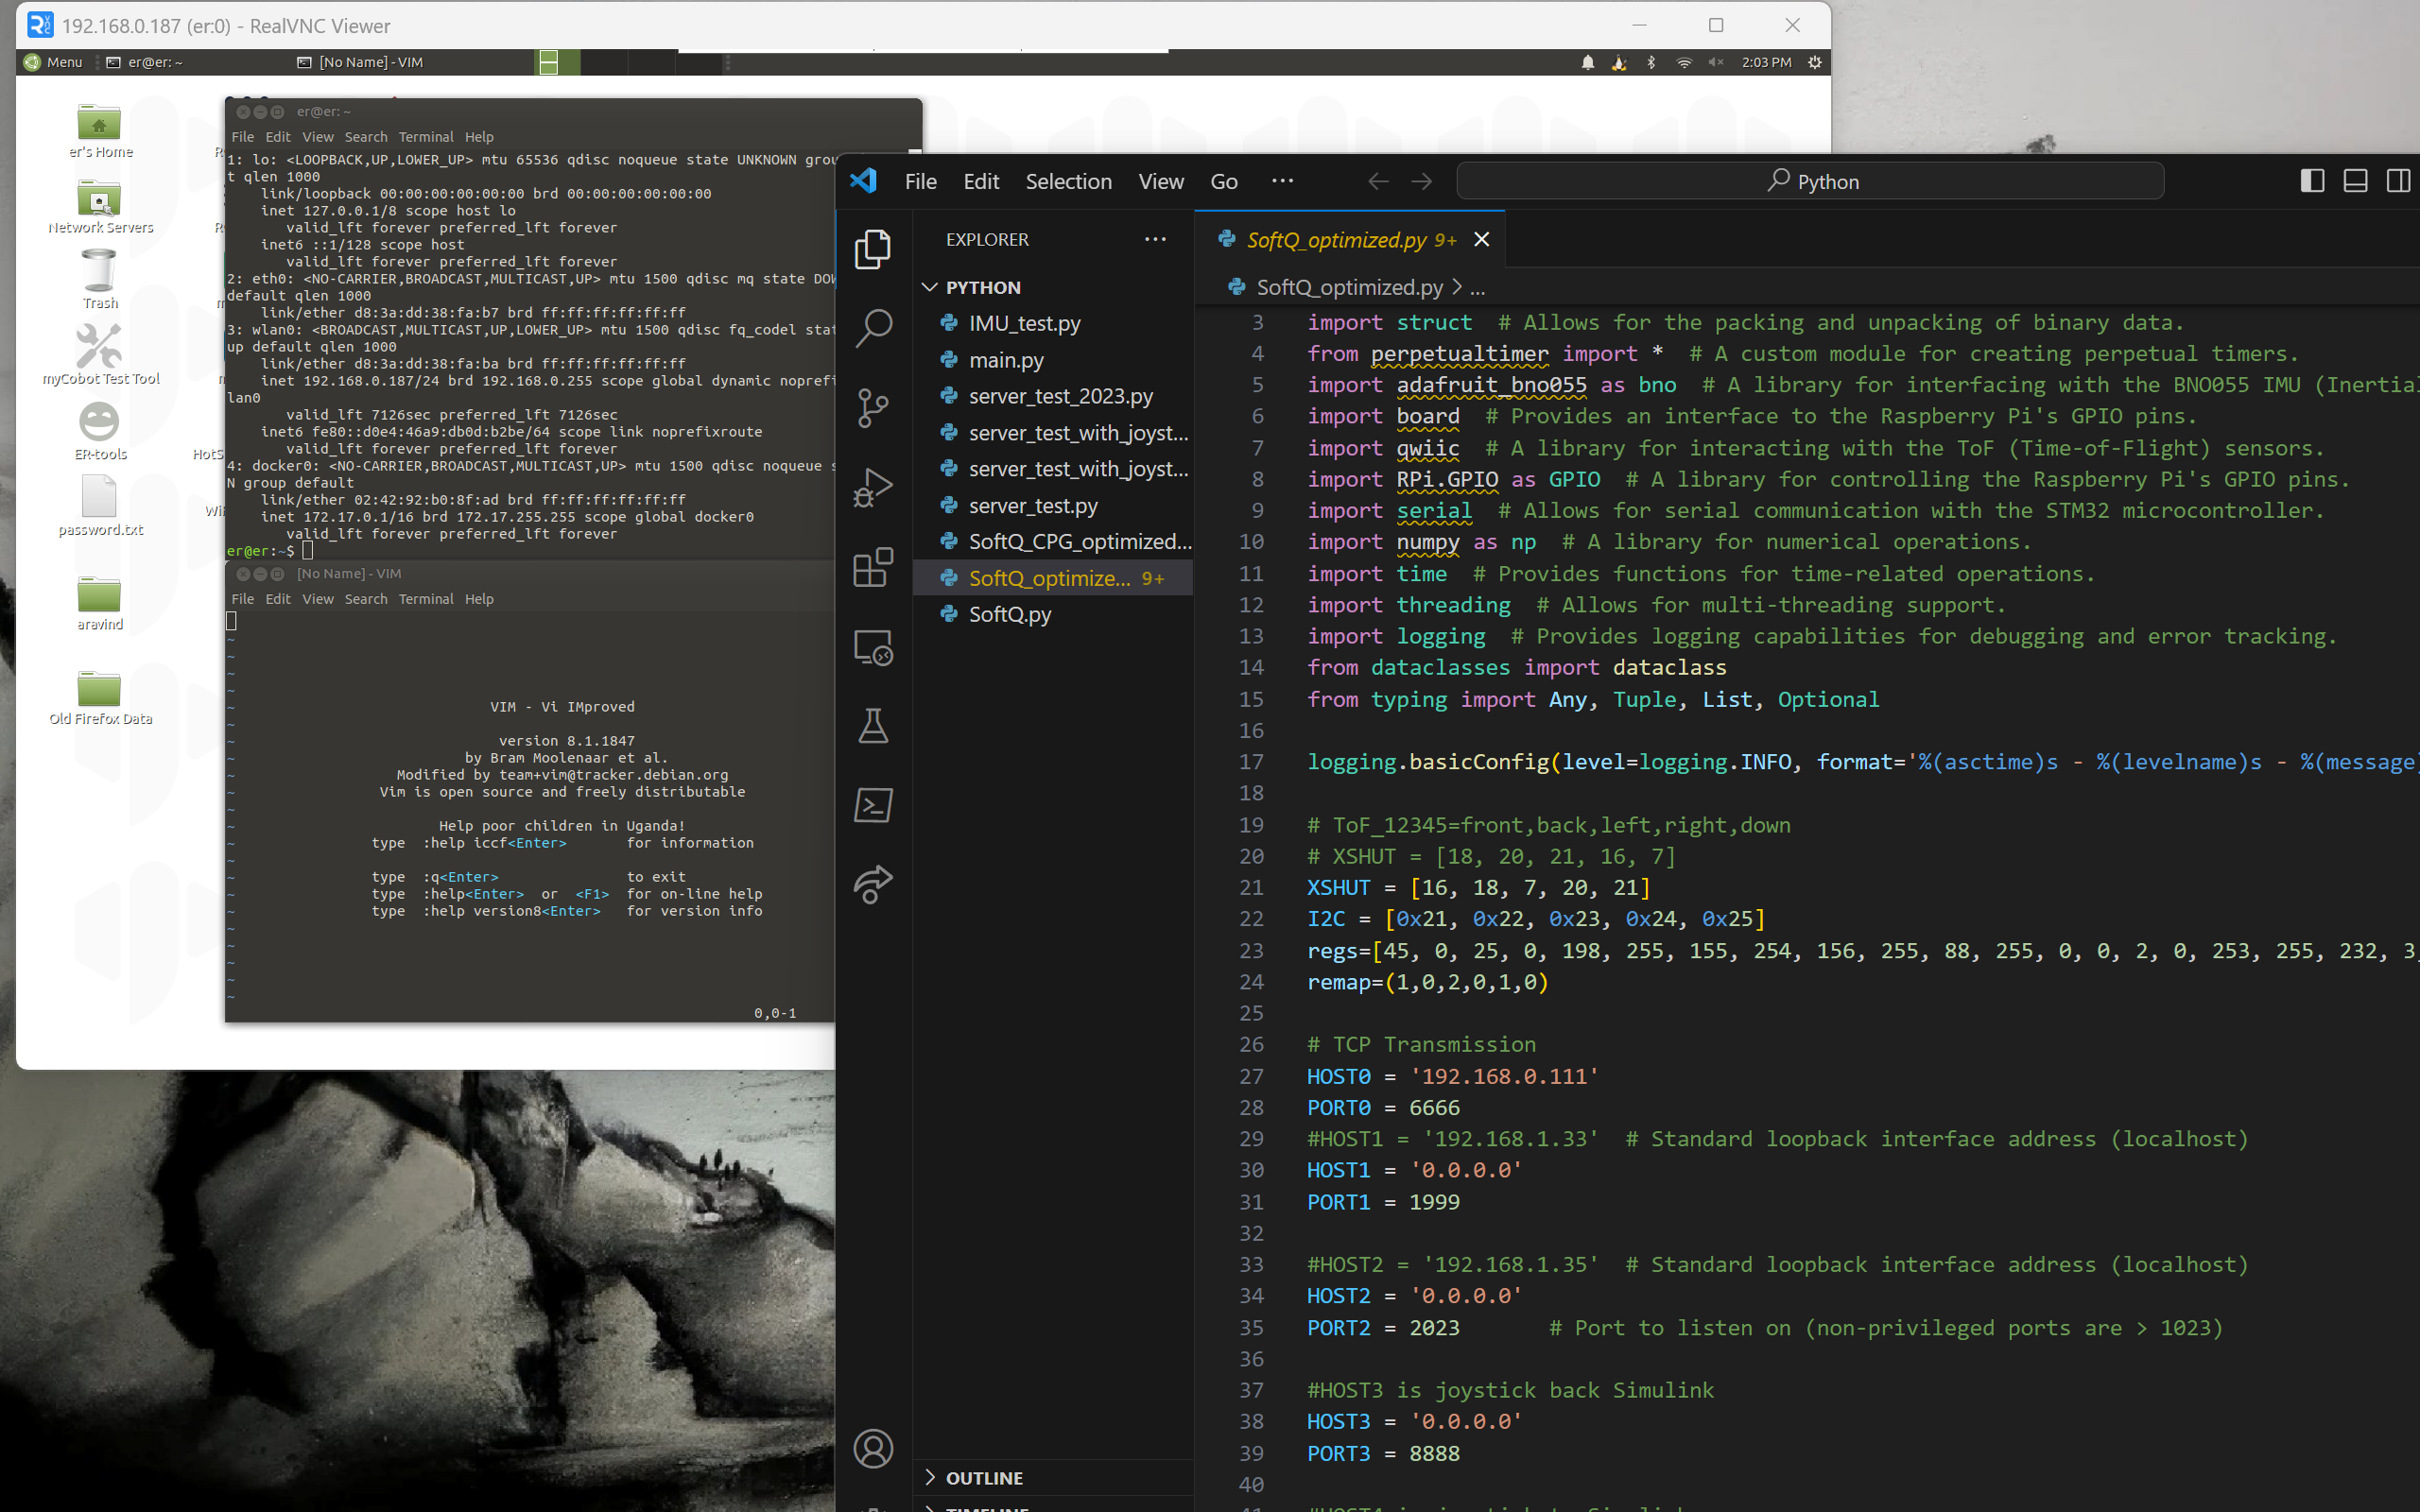
\includegraphics[width=0.75\linewidth]{Figures/work_flow.png}
\end{figure}

\begin{itemize}
    \item Check the IP address from the robot by typing 'ip addr' in the Terminal of robot. See the figure below.
\begin{figure}[H]
    \centering
    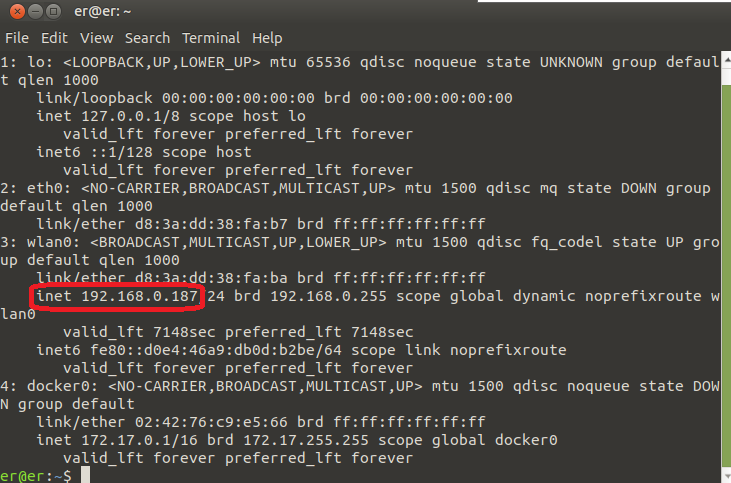
\includegraphics[width=0.6\linewidth]{Figures/ip_robot.png}
\end{figure}
    \item Check the IP address from the configuration page of routers. The default address for TP-Link router is '192.168.0.1'. See the figure below.
\begin{figure}[H]
    \centering
    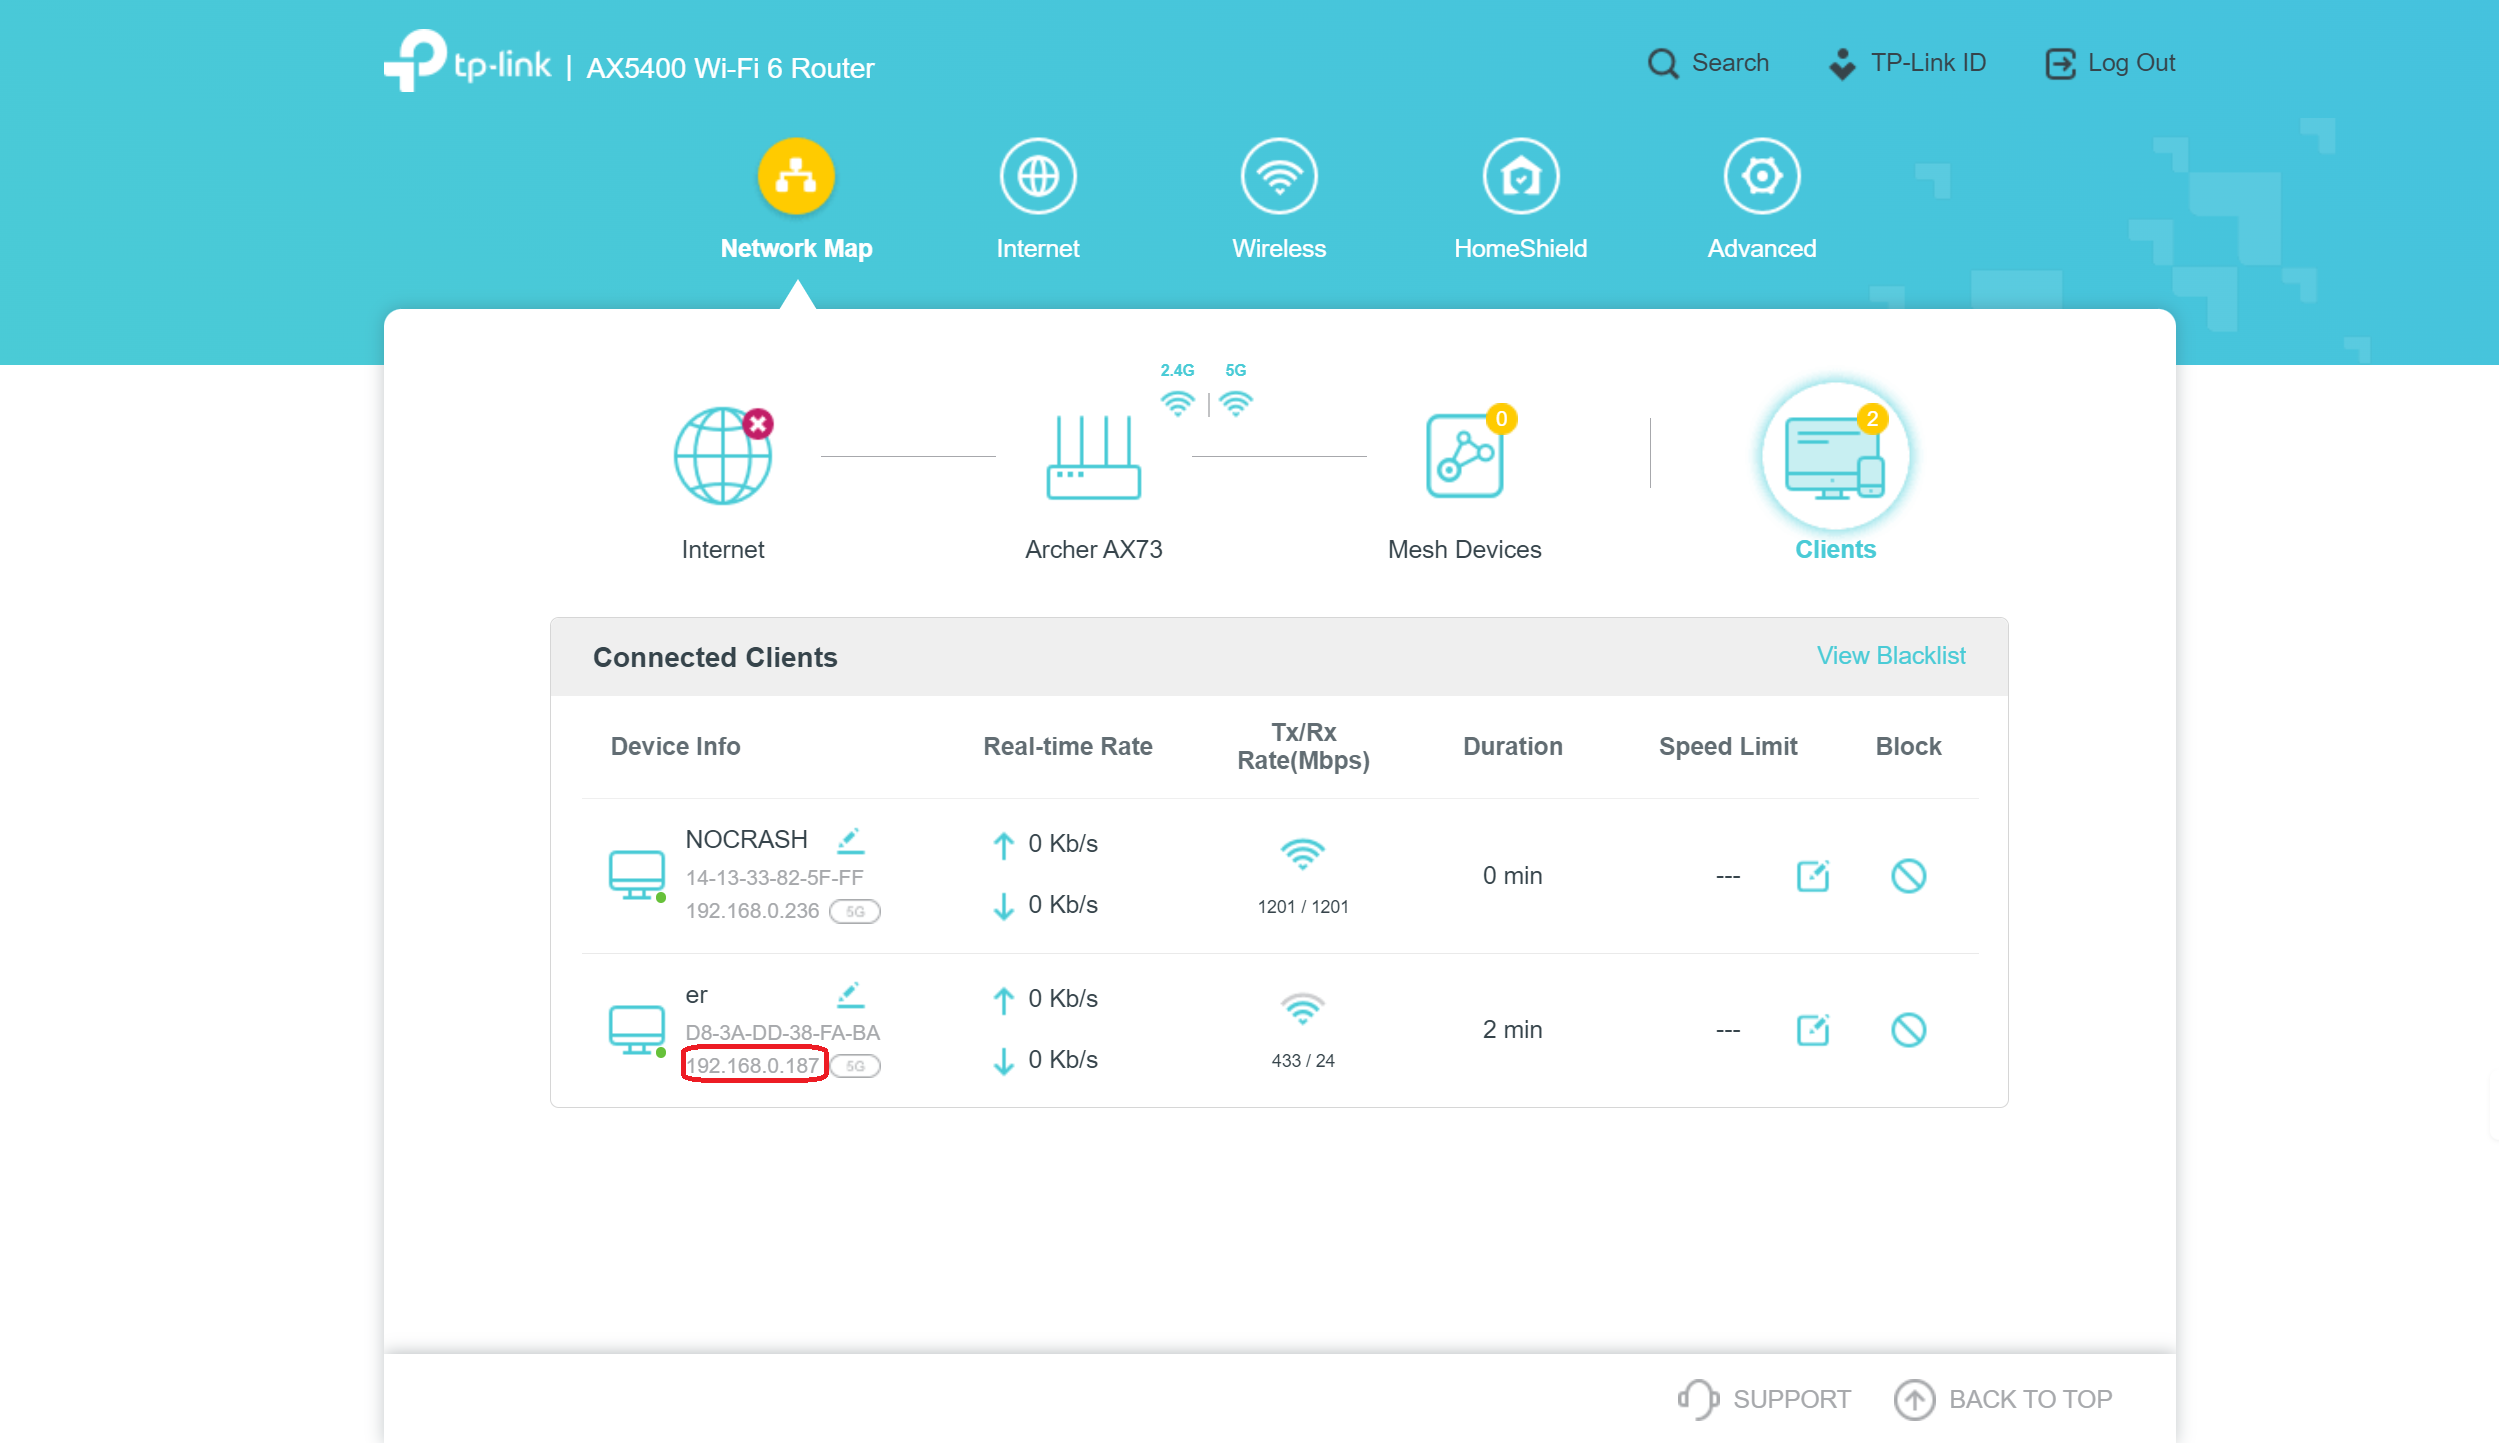
\includegraphics[width=0.75\linewidth]{Figures/ip_router.png}
\end{figure}
\end{itemize}

After obtaining the IP address of the robot, input it into VNC to establish remote access. This allows you to work on a more powerful computer than the Raspberry Pi, where the firmware is executed.

\textbf{Dobot Nova 5}
The procedure for connecting to the large robotic arm differs slightly, as it utilizes industry-standard software developed by Dobot, known as DobotStudio Pro. Before using the robot, you need to connect to the Wi-Fi network that the robot broadcast itself, and then connect to '192.168.5.1' to have full features that software can do. Additionally, there is an alternative address, '192.168.1.6', designated for data exchange. Connecting to this address allows the robot to execute commands, but the visual animation of the arm will be disabled.
\begin{figure}[H]
    \centering
    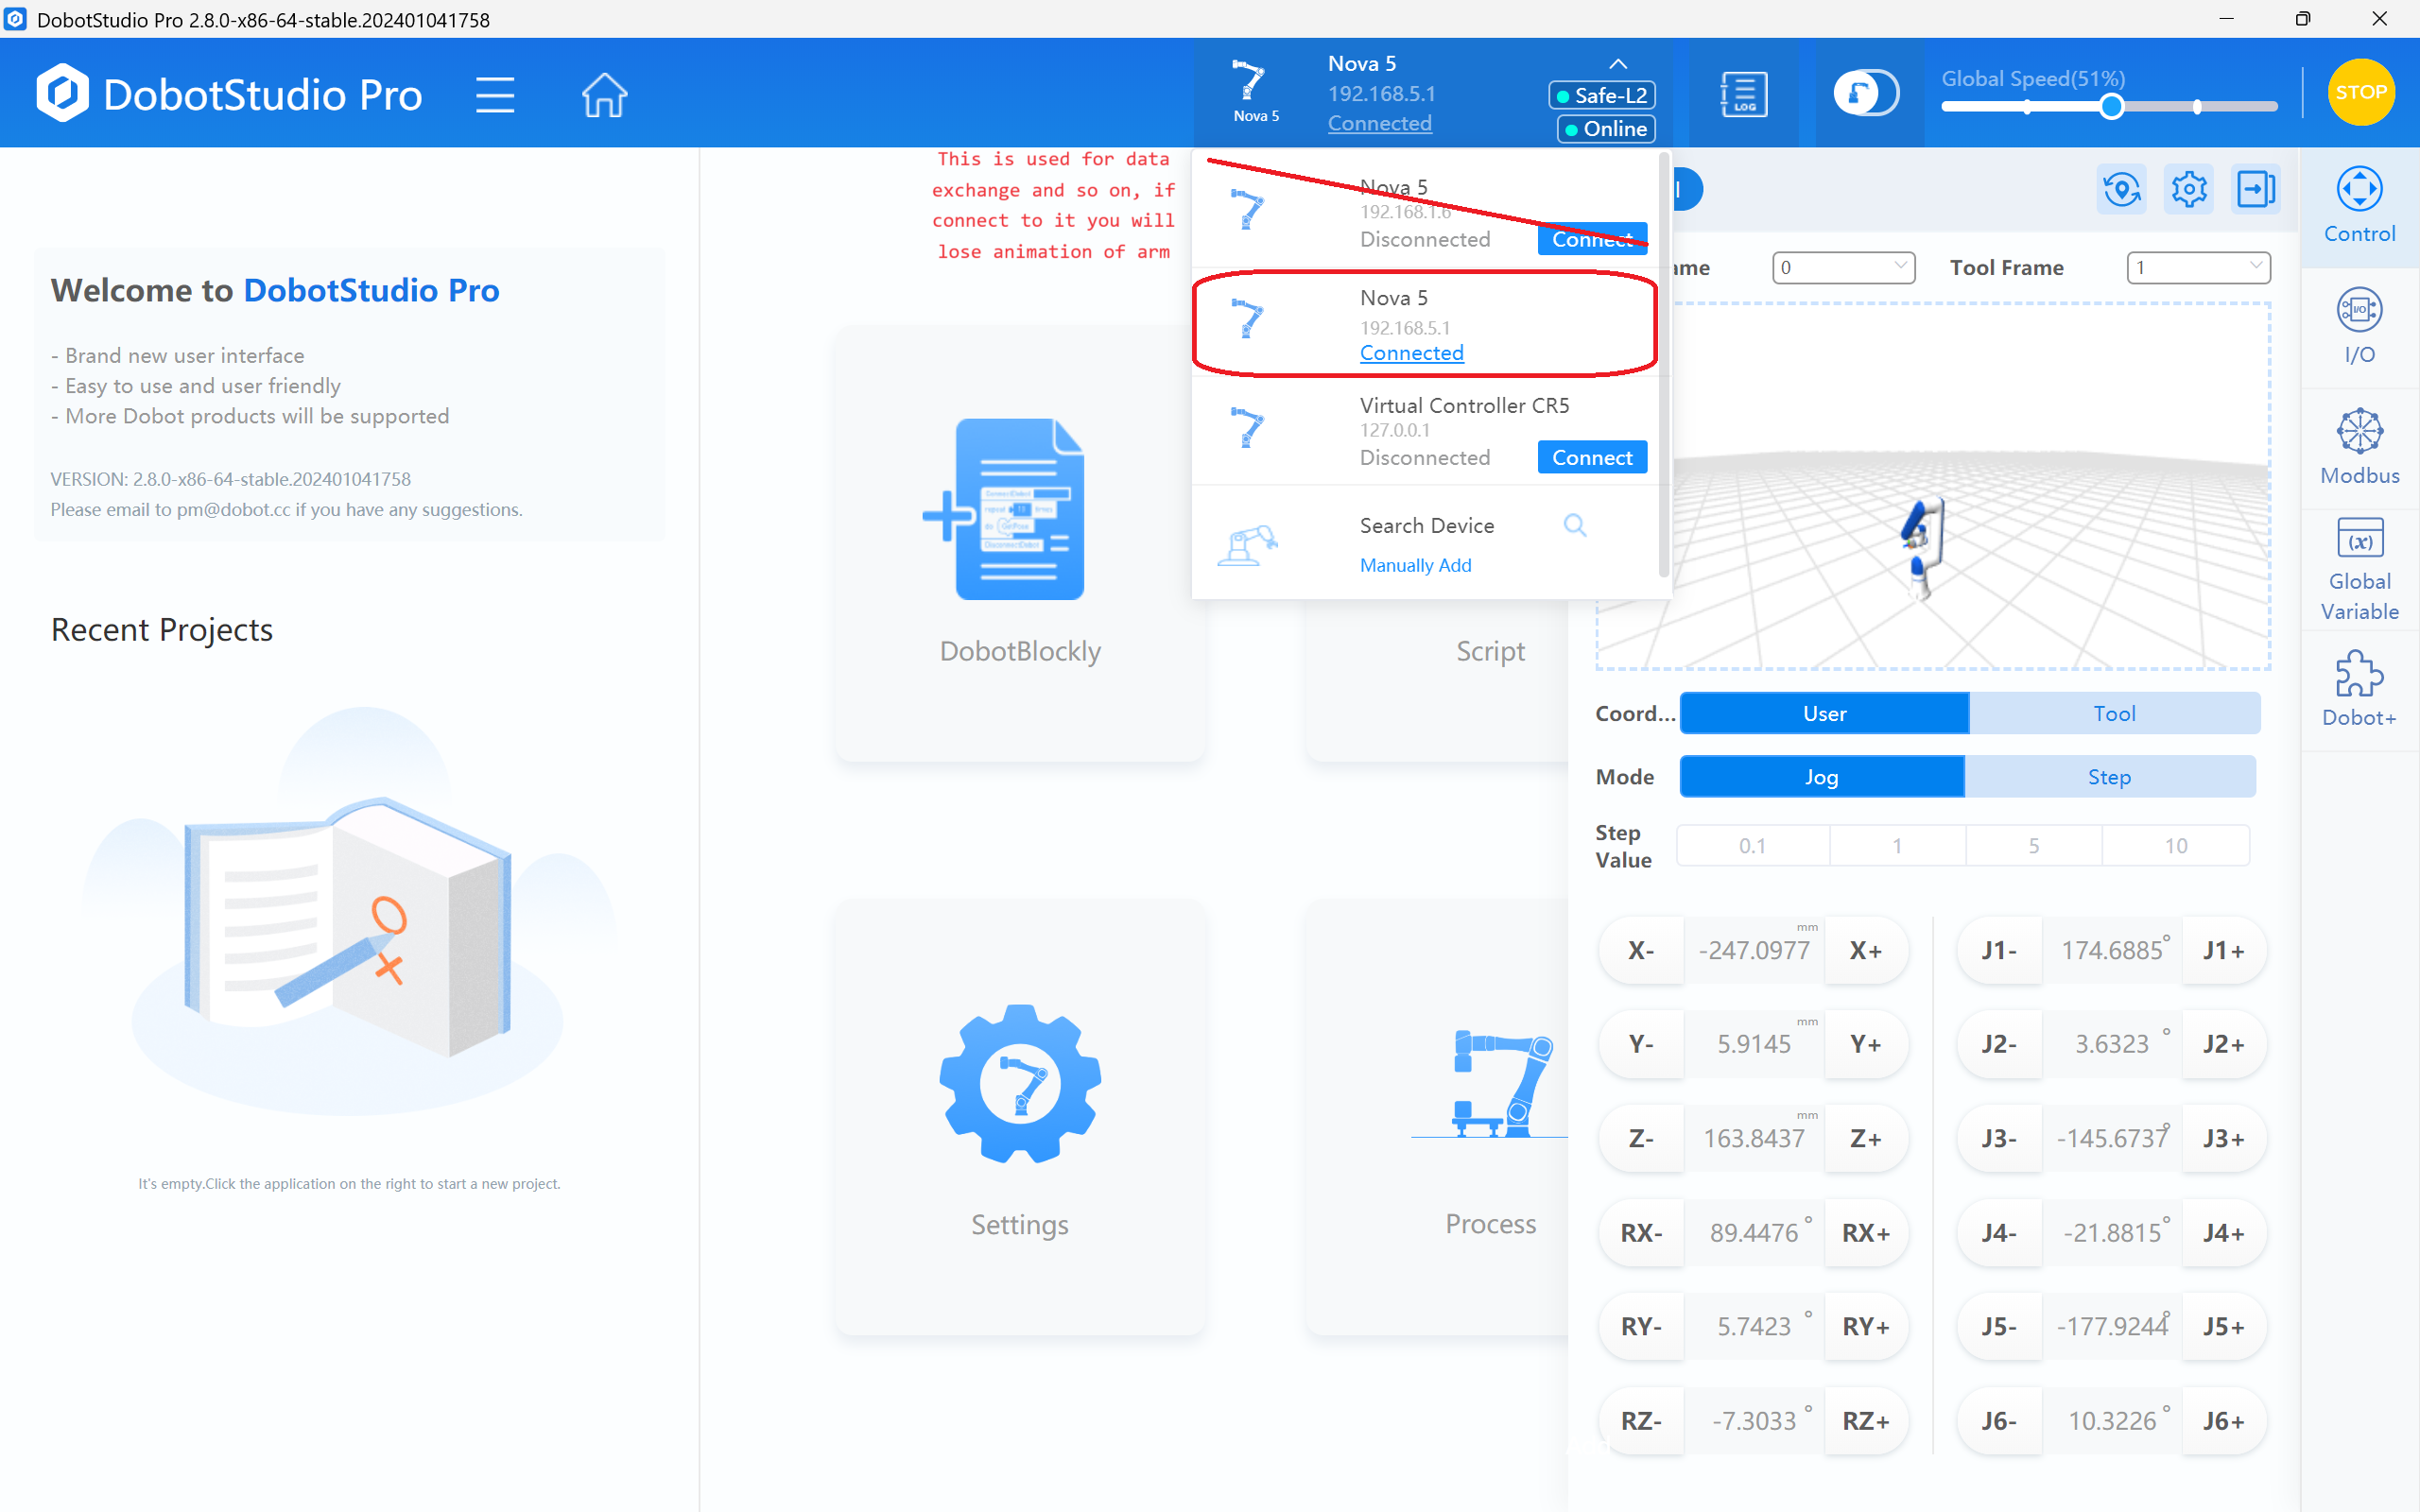
\includegraphics[width=0.8\linewidth]{Figures/dobot_gui.png}
\end{figure}

\newpage
\section*{Routers}
We have two routers in the lab. 

\begin{minipage}[t]{0.5\linewidth}
    TP-Link AX73 Router is configured to have 
    \begin{itemize}
        \item Wi-Fi network: 'Robot\_All'
        \item Password: CPS104264 
        \item Configuration page: 192.168.0.1
        \item Admin password: CPS104264
    \end{itemize}
\end{minipage}%
\begin{minipage}[t]{0.5\linewidth}
    TP-Link TL-WR841N is is configured to have 
    \begin{itemize}
        \item Wi-Fi network: 'Robot\_Net'
        \item Password: 12345678 
        \item Configuration page: 192.168.0.1
        \item Admin password: 123456
    \end{itemize}
\end{minipage}


\section*{Lab Computer}

\end{document}